\documentclass{beamer}
\usepackage[utf8]{inputenc}

\usetheme{Madrid}
\usecolortheme{default}
\usepackage{amsmath,amssymb,amsfonts,amsthm}
\usepackage{txfonts}
\usepackage{tkz-euclide}
\usepackage{listings}
\usepackage{adjustbox}
\usepackage{array}
\usepackage{tabularx}
\usepackage{gvv}
\usepackage{lmodern}
\usepackage{circuitikz}
\usepackage{tikz}
\usepackage{graphicx}

\setbeamertemplate{page number in head/foot}[totalframenumber]

\usepackage{tcolorbox}
\tcbuselibrary{minted,breakable,xparse,skins}



\definecolor{bg}{gray}{0.95}
\DeclareTCBListing{mintedbox}{O{}m!O{}}{%
  breakable=true,
  listing engine=minted,
  listing only,
  minted language=#2,
  minted style=default,
  minted options={%
    linenos,
    gobble=0,
    breaklines=true,
    breakafter=,,
    fontsize=\small,
    numbersep=8pt,
    #1},
  boxsep=0pt,
  left skip=0pt,
  right skip=0pt,
  left=25pt,
  right=0pt,
  top=3pt,
  bottom=3pt,
  arc=5pt,
  leftrule=0pt,
  rightrule=0pt,
  bottomrule=2pt,
  toprule=2pt,
  colback=bg,
  colframe=orange!70,
  enhanced,
  overlay={%
    \begin{tcbclipinterior}
    \fill[orange!20!white] (frame.south west) rectangle ([xshift=20pt]frame.north west);
    \end{tcbclipinterior}},
  #3,
}
\lstset{
    language=C,
    basicstyle=\ttfamily\small,
    keywordstyle=\color{blue},
    stringstyle=\color{orange},
    commentstyle=\color{green!60!black},
    numbers=left,
    numberstyle=\tiny\color{gray},
    breaklines=true,
    showstringspaces=false,
}
%------------------------------------------------------------

\title
{3.2.19}
\date{September 2,2025}
\author 
{AI25BTECH11003 - Bhavesh Gaikwad}



\begin{document}


\frame{\titlepage}
\begin{frame}{Question}
Two sides of a triangle are of lengths 5cm and 1.5cm. The length of the third side of the triangle cannot be\\
a) 3.6 cm\\
b) 4.1 cm\\
c) 3.8 cm\\
d) 3.4 cm\\
\end{frame}


\begin{frame}[fragile]
    \frametitle{Theoretical Solution}
 Assume Triangle ABC with $\norm{\vec{AC}} = b = 1.5cm, \; \norm{\vec{AB}} = c = 5cm, \; \norm{\vec{BC}} = a$ \\
and Angle A = $\alpha$\\
Let $\vec{A} = \myvec{ 0 \\ 0}$\\
Therefore, $\vec{C} = \myvec{b \\ 0} = \myvec{ 1.5 \\ 0}$ and $\vec{B} = \myvec{c\cos\alpha \\ c\sin\alpha} = \myvec{5\cos\alpha \\ 5\sin\alpha}$\\\\


By Cosine Law,
\begin{equation}
a^2 = b^2 + c^2 - 2bc\cos\alpha
\end{equation}

\begin{align}
a^2 = 27.25 - 15\cos\alpha
\end{align}

\begin{equation}
\cos\alpha = \frac{27.25 - a^2}{15}
\end{equation}
\end{frame}

\begin{frame}[fragile]
    \frametitle{Theoretical Solution}
    Option (A) a = 3.6cm
\begin{equation}
    \cos\alpha = \dfrac{27.25 - 12.96}{15} = \dfrac{14.29}{15}
\end{equation}

 \begin{equation}
\Rightarrow \, \alpha = 17.7^\circ     
 \end{equation}

\begin{figure}[htbp]
    \centering
    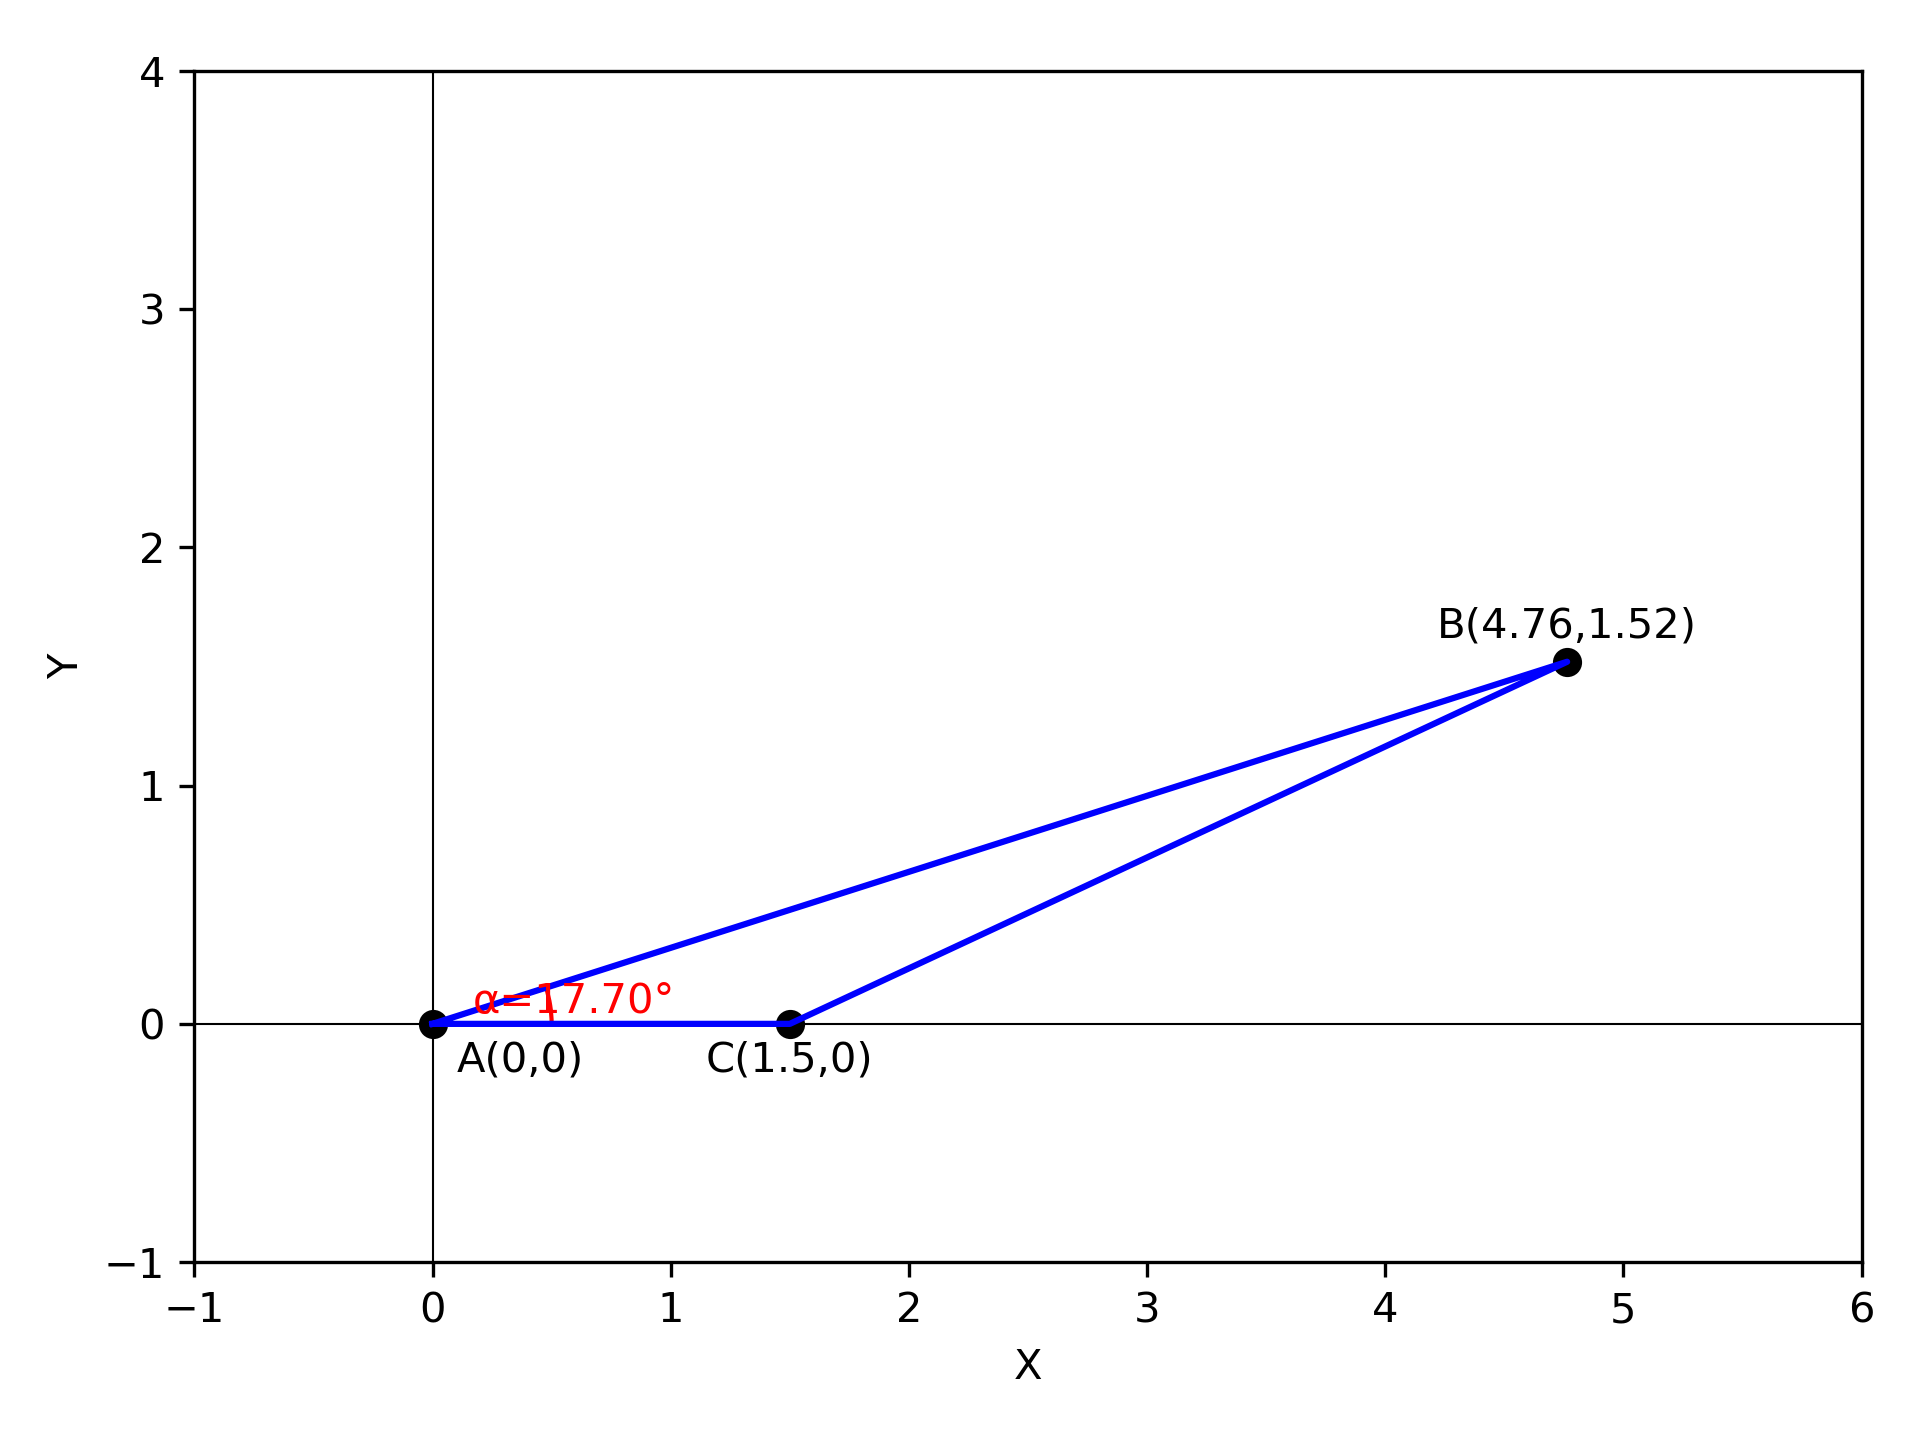
\includegraphics[width=0.6\columnwidth]{figs/fig1.png}
    \caption{Triangle ABC of Option (A)}
    \label{fig:placeholder}
\end{figure}
\end{frame}

\begin{frame}[fragile]
    \frametitle{Theoretical Solution}
Option (B) a = 4.1cm
\begin{equation}
    \cos\alpha = \dfrac{27.25 - 16.81}{15} = \dfrac{10.44}{15}
\end{equation}

 \begin{equation}
\Rightarrow \, \alpha = 45.89^\circ     
 \end{equation}

\begin{figure}[htbp]
    \centering
    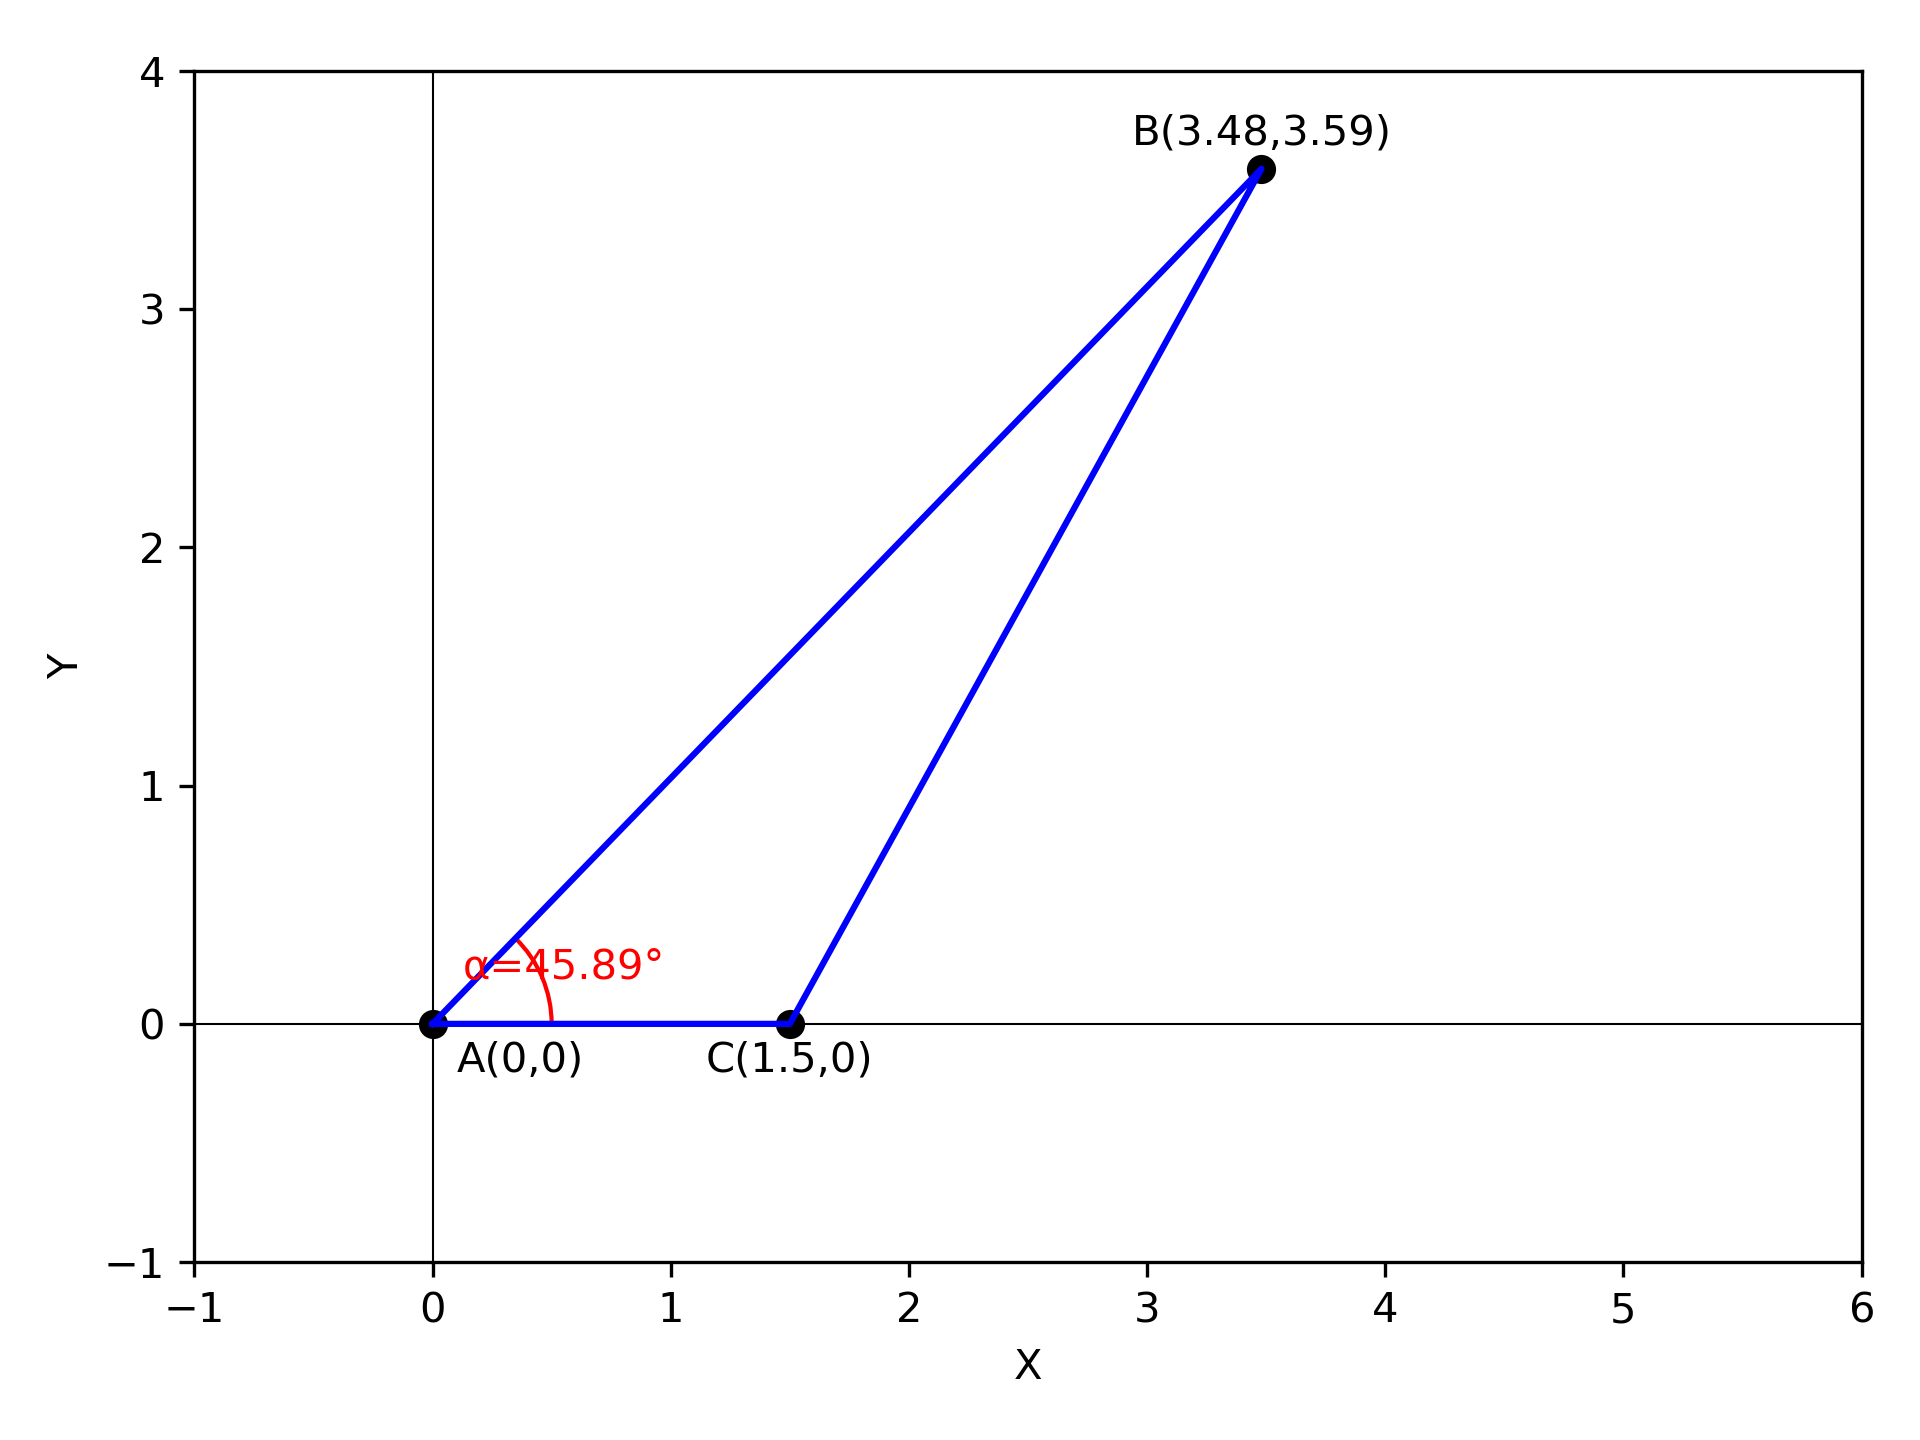
\includegraphics[width=0.6\columnwidth]{figs/fig2.png}
    \caption{Triangle ABC of Option (B)}
    \label{fig:placeholder}
\end{figure}
\end{frame}

\begin{frame}[fragile]
    \frametitle{Theoretical Solution}
    Option (C) a = 3.8cm
\begin{equation}
    \cos\alpha = \dfrac{27.25 - 14.44}{15} = \dfrac{12.81}{15}
\end{equation}

 \begin{equation}
\Rightarrow \, \alpha = 31.35^\circ     
 \end{equation}

\begin{figure}[htbp]
    \centering
    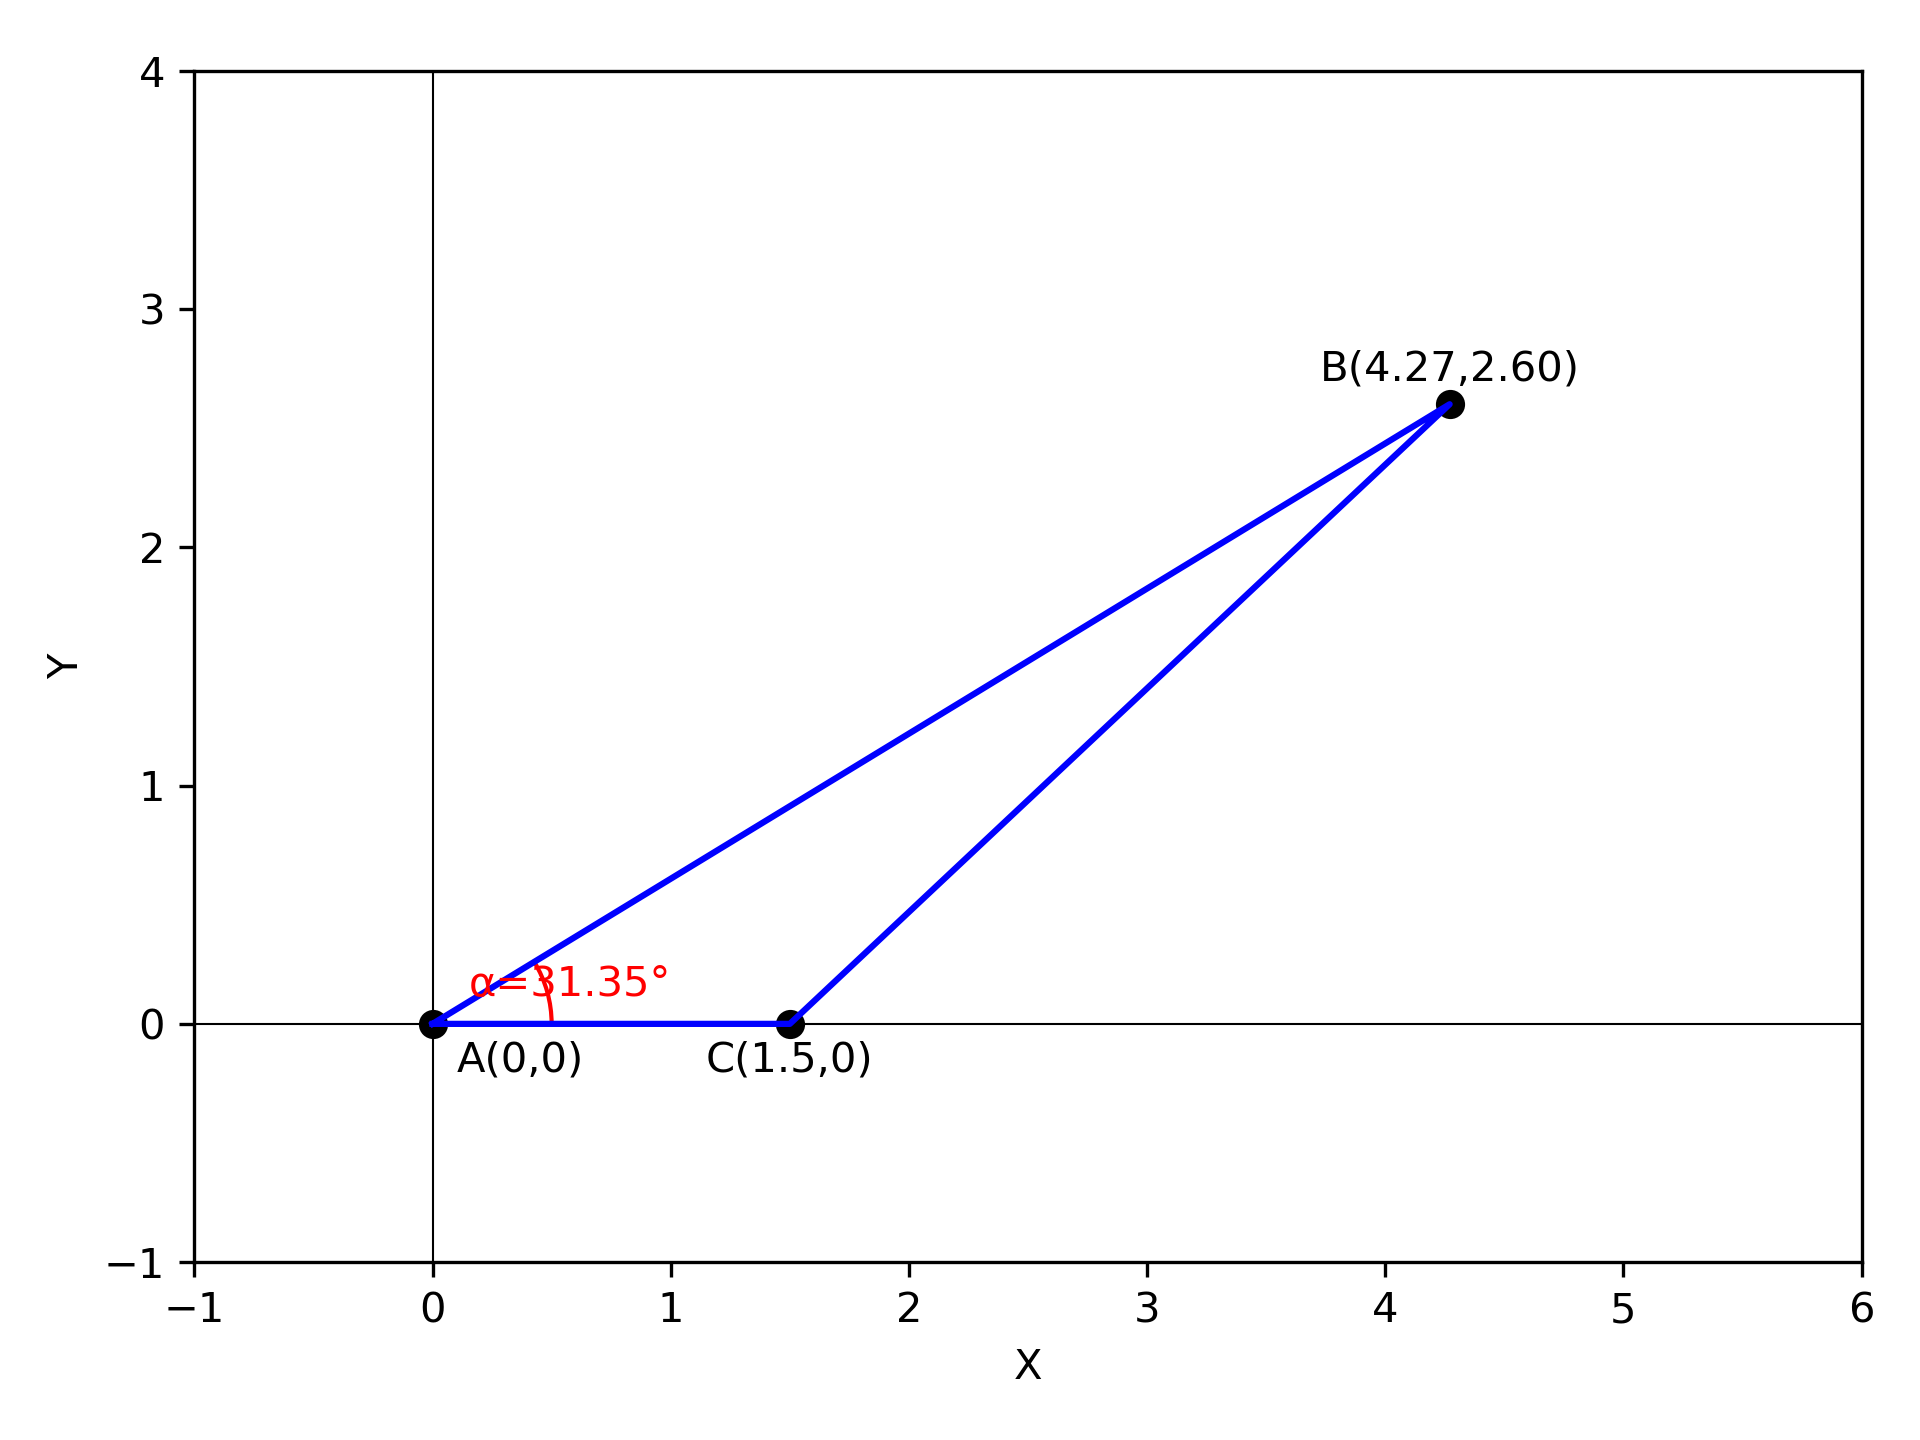
\includegraphics[width=0.6\columnwidth]{figs/fig3.png}
    \caption{Triangle ABC of Option (C)}
    \label{fig:placeholder}
\end{figure}
\end{frame}

\begin{frame}[fragile]
    \frametitle{Theoretical Solution}
    Option (D) a = 3.4cm
\begin{equation}
    \cos\alpha = \dfrac{27.25 - 11.56}{15} = \dfrac{15.69}{15}
\end{equation}
\begin{equation}
    \text{Here, } \cos\alpha > 1 \text{ which is not possible}
\end{equation}

\begin{figure}[htbp]
    \centering
    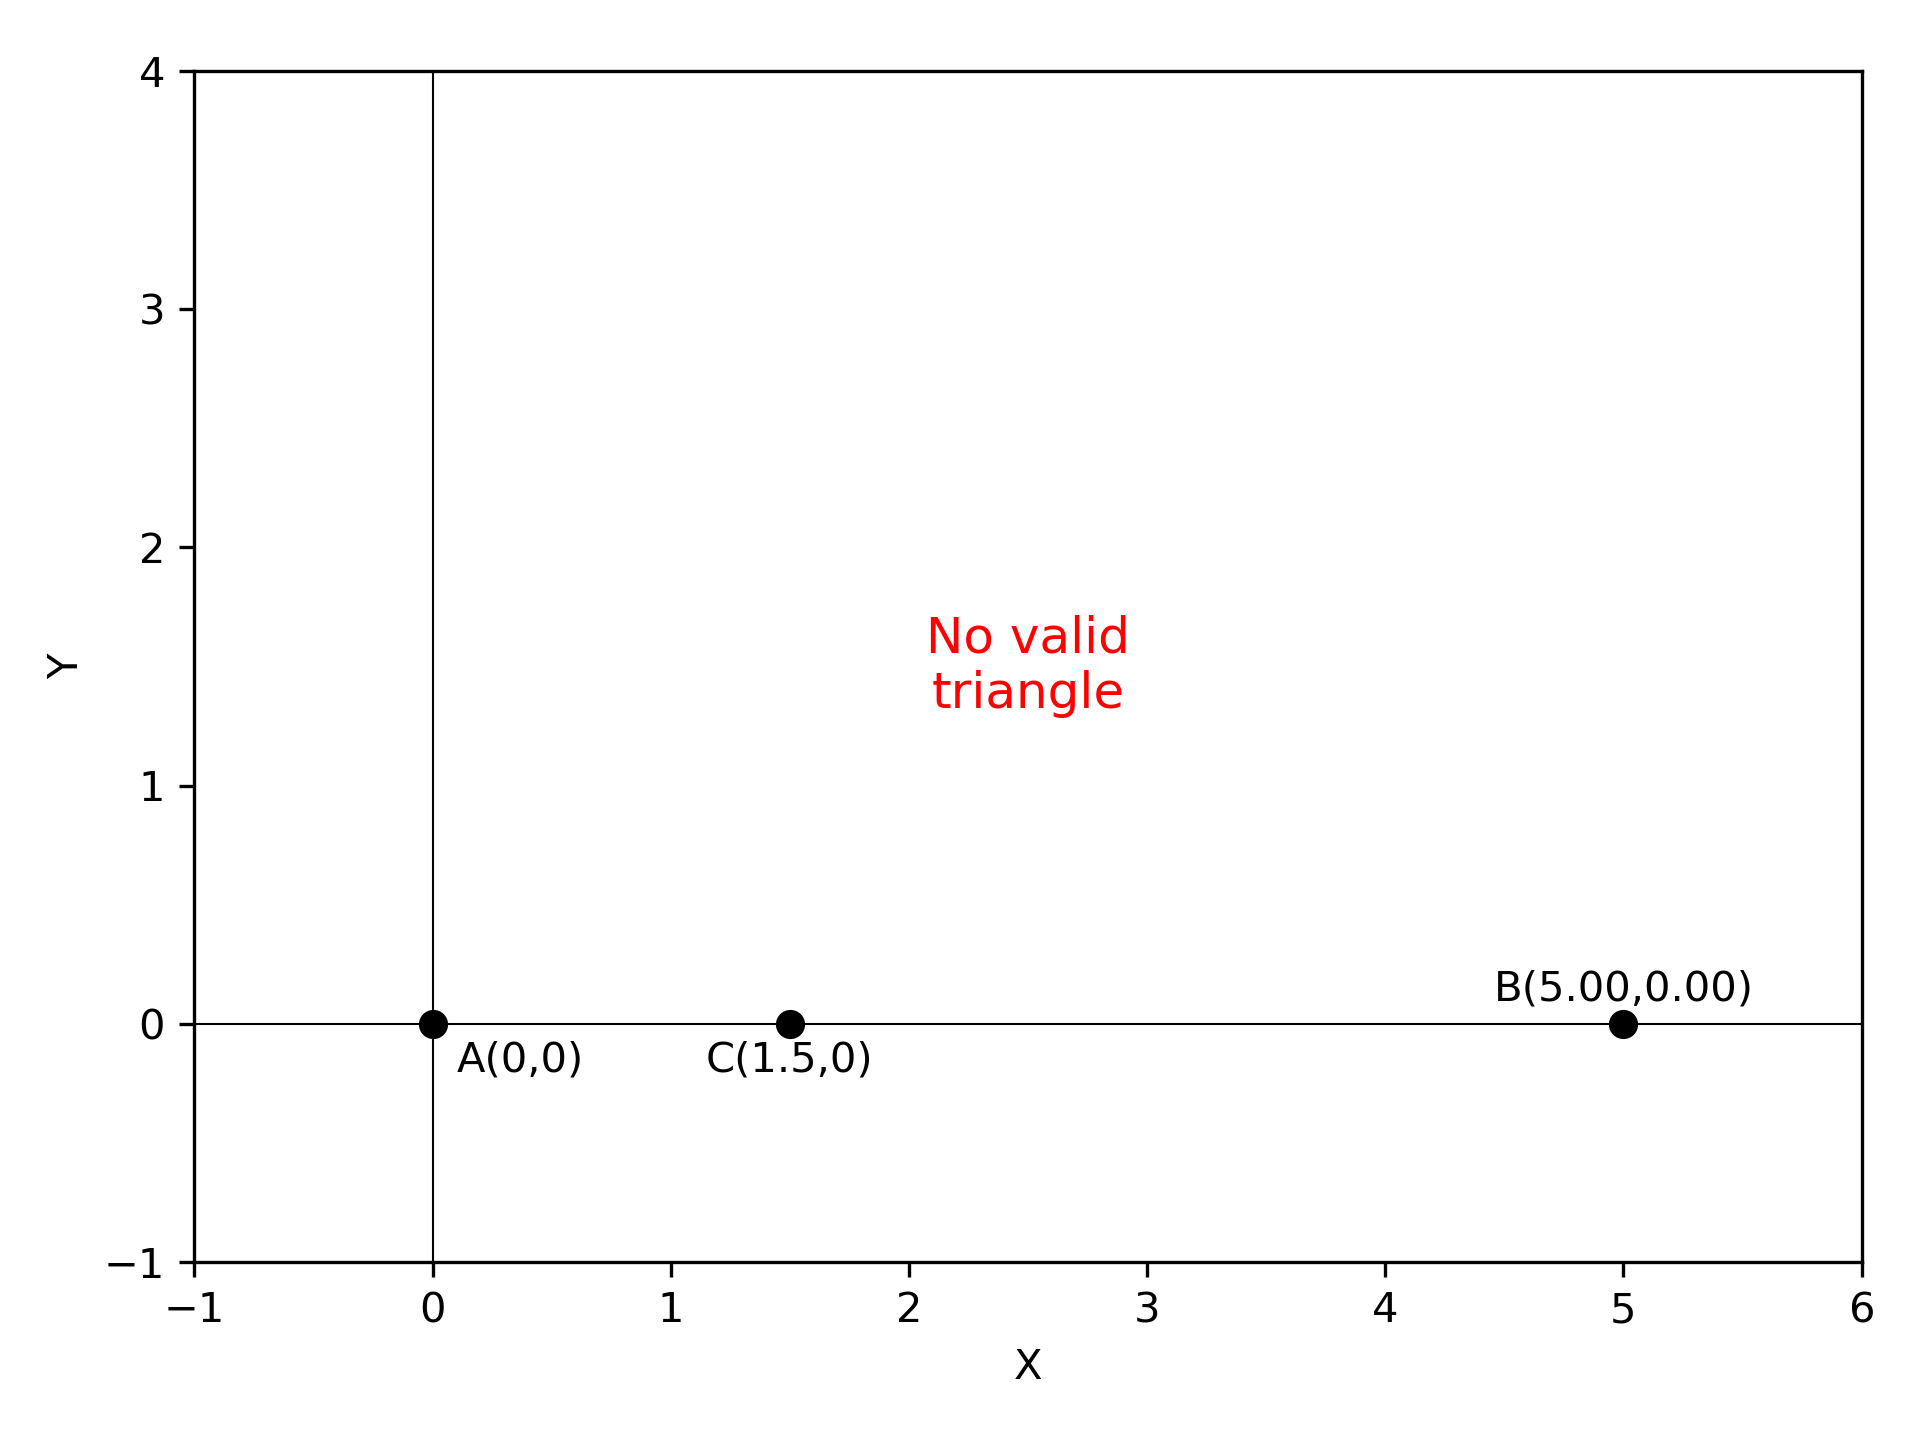
\includegraphics[width=0.6\columnwidth]{figs/fig4.png}
    \caption{Image of Option (D)}
    \label{fig:placeholder}
\end{figure}
\end{frame}

\begin{frame}[fragile]
    \frametitle{Theoretical Solution}\
    \begin{align*}
    \boxed{\text{Thus, Option (D) is incorrect.}}
\end{align*}
\end{frame}



\end{document}